\section{Gadgets}
\label{gadgets}


% { \tt Gadget}( $\left\langle \text{Input} \right\rangle, \left\langle \text{Output}  \right\rangle$ )

\newcommand{\warpunit}{{\tt Warp\_Unit}}
\newcommand{\prewarp}{{\tt Pre\_Warp}}
\newcommand{\firstwarp}{{\tt First\_Warp}}
\newcommand{\warpbridge}{{\tt Warp\_Bridge}}
\newcommand{\secondwarp}{{\tt Second\_Warp}}
\newcommand{\postwarp}{{\tt Post\_Warp}}

\newcommand{\dtop}{{\tt Digit\_Top}}
\newcommand{\dwriter}{{\tt Digit\_Writer}}
\newcommand{\dreader}{{\tt Digit\_Reader}}

\newcommand{\returnfromdonereadnextrow}{{\tt Return\_From\_Digit1\_Read\_Next\_Row}}
\newcommand{\returnfromdtworeadnextrow}{{\tt Return\_From\_Digit2\_Read\_Next\_Row}}
\newcommand{\returnfromdthreereadnextrow}{{\tt Return\_From\_Digit3\_Read\_Next\_Row}}

\newcommand{\returnfromdonereaddtwo}{{\tt Return\_From\_Digit1\_Read\_Digit2}}
\newcommand{\returnfromdonereaddtwocasetwo}{{\tt Return\_From\_Digit1\_Read\_Digit2\_Case2}}
\newcommand{\returnfromdtworeaddthree}{{\tt Return\_From\_Digit2\_Read\_Digit3}}
\newcommand{\returnfromdthreereaddone}{{\tt Return\_From\_Digit3\_Read\_Digit1}}

\newcommand{\inc}{{\tt op}}

\newcommand{\dtopdonecaseone}{{\tt Digit\_Top\_Digit1\_Case1}}
\newcommand{\dtopdonecasetwo}{{\tt Digit\_Top\_Digit1\_Case2}}
\newcommand{\dtopdtwocasetwo}{{\tt Digit\_Top\_Digit2\_Case2}}
\newcommand{\dtopcasethree}{{\tt Digit\_Top\_Case3}}

% todo: fix wording
When describing a special case, i.e. ``digit $x$ -- case $y$'', whatever follows
will only apply to the MSR (due to each case only affecting the MSR.)

\subsection{ Counter Unit }


    \subsubsection{ Digit readers }
        \begin{itemize}
            \item For each $i = 1,2,3$,
                           $j = 1,\ldots,l-1$
                           $u \in \{0, 1\}^j$,
                           and each $\inc \in \{{\tt increment}, {\tt copy} \}$

                \begin{itemize}
                \item Create
                    $\begin{aligned}[t]
                        \dreader(& \left\langle {\tt DigitReader}, i, u, \inc \right\rangle, \\
                                 & \left\langle {\tt DigitReader}, i, 0u, \inc \right\rangle, \\
                                 & \left\langle {\tt DigitReader}, i, 1u, \inc \right\rangle \;)
                    \end{aligned}$
                \end{itemize}

            \item For each $i = 1,2,3$ and each $\inc \in \{{\tt increment}, {\tt copy} \}$

                \begin{itemize}
                \item Create
                    $\begin{aligned}[t]
                        \dreader(& \left\langle {\tt DigitReader}, i, \lambda, \inc \right\rangle, \\
                                 & \left\langle {\tt DigitReader}, i, 0, \inc \right\rangle, \\
                                 & \left\langle {\tt DigitReader}, i, 1, \inc \right\rangle \;)
                    \end{aligned}$
                \end{itemize}



        \end{itemize}

        \begin{figure}[H]
            \centering
            \begin{subfigure}[t]{0.2\textwidth}
                \centering
                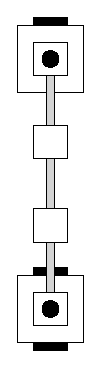
\includegraphics[width=0.2\textwidth]{read/read_0}
                \caption{\label{fig:read/read_1} Counter\_Read\_0}
            \end{subfigure}%
            ~
            \begin{subfigure}[t]{0.2\textwidth}
                \centering
                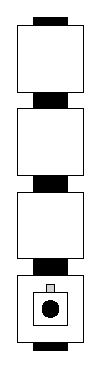
\includegraphics[width=0.2\textwidth]{read/read_1}
                \caption{\label{fig:read/read_1} Counter\_Read\_1}
            \end{subfigure}%
        \end{figure}

    % For each digit length L
\subsubsection{ Warping }

% For each index in 1, 2, 3, and carry in 0,1
    For each $i = 1, 2, 3$, $u \in \{0, 1\}^l$, and each $\inc \in \{ {\tt increment, copy } \}$
    (note: since this might not be the correct notation, in words: do this for each binary encoded digit of length $l$,
    for each digit-region index, and both copy/increment signals)



    \begin{itemize}

        \item Create
        $\begin{aligned}[t]
            \prewarp(& \left\langle {\tt PreWarp},   i, u, \inc \right\rangle, \\
                     & \left\langle {\tt FirstWarp}, i, u, \inc \right\rangle \;)
        \end{aligned}$
        \vspace{.5cm}



        \begin{figure}[H]
            \begin{subfigure}[t]{0.2\textwidth}
                \centering
                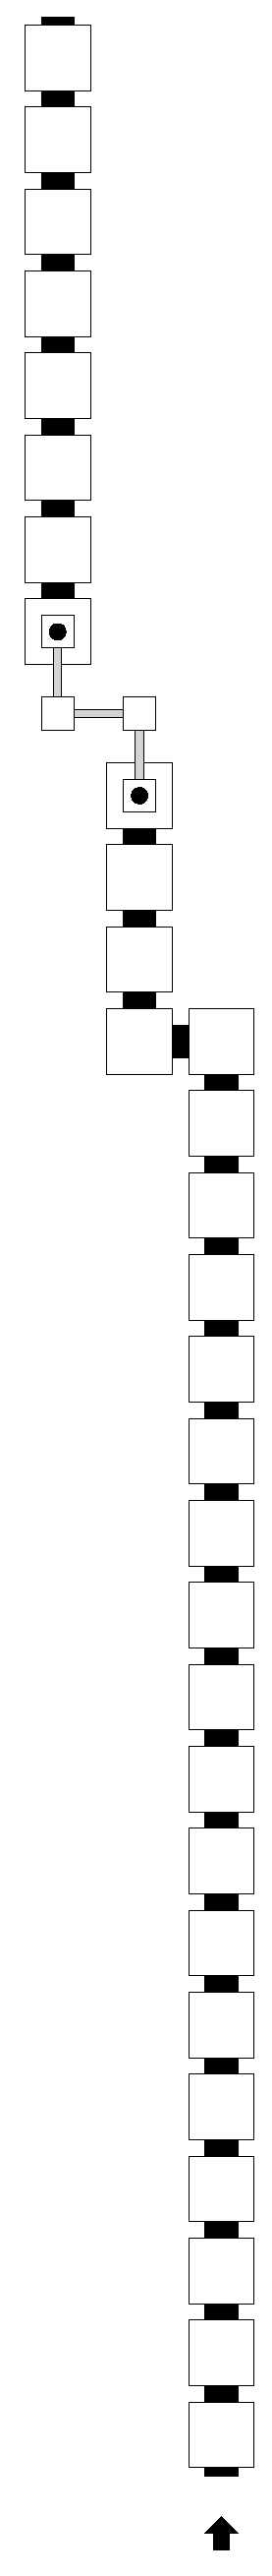
\includegraphics[width=0.2\textwidth]{warping/pre_warp_general}
                \caption{\label{fig:warping/pre_warp_general} General }
            \end{subfigure}%
            ~
            \begin{subfigure}[t]{0.2\textwidth}
                \centering
                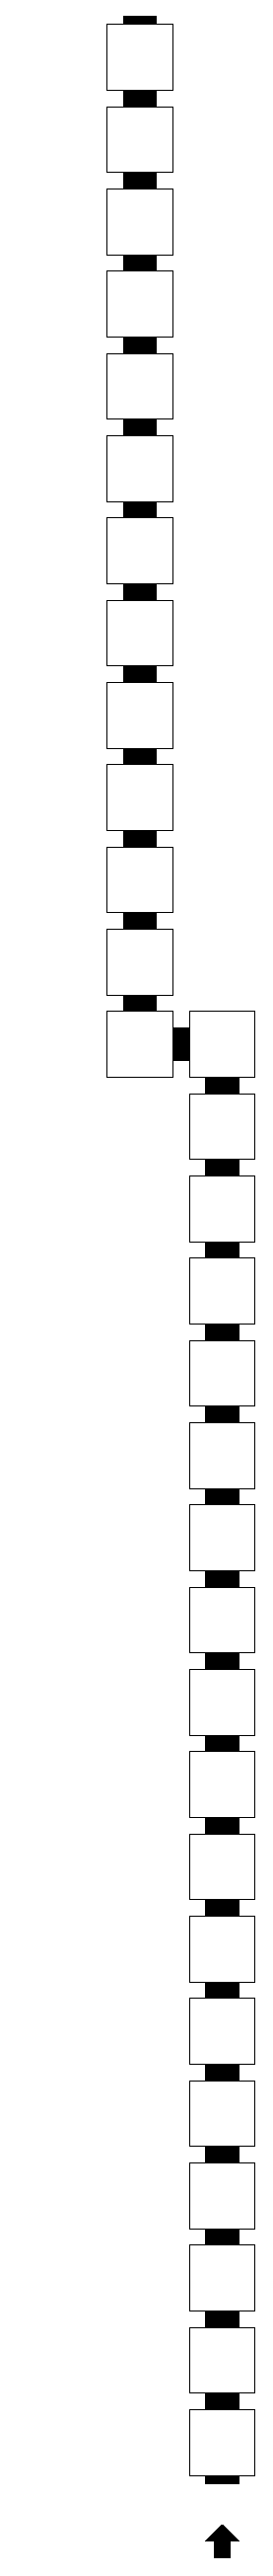
\includegraphics[width=0.2\textwidth]{warping/pre_warp_case1_digit1_msr}
                \caption{\label{fig:warping/pre_warp_case1_digit1_msr} Digit 1 -- Case 1}
            \end{subfigure}%
            ~
            \begin{subfigure}[t]{0.2\textwidth}
                \centering
                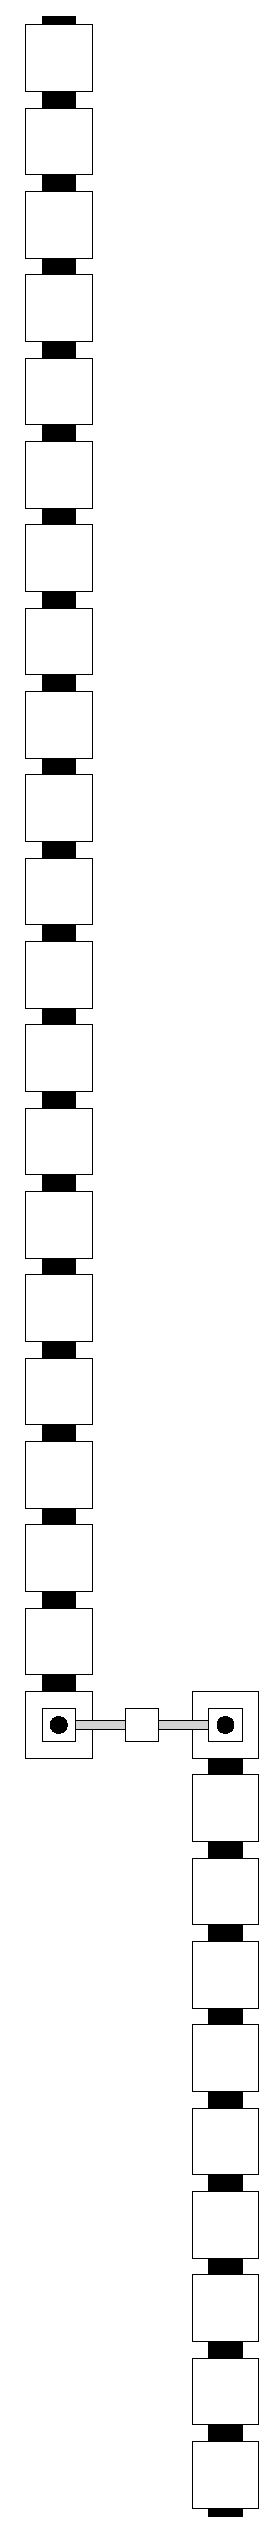
\includegraphics[width=0.2\textwidth]{warping/pre_warp_case2_digit1_msr}
                \caption{\label{fig:warping/pre_warp_case2_digit1_msr} Digit 1 -- Case 2}
            \end{subfigure}%
            ~
            \begin{subfigure}[t]{0.2\textwidth}
                \centering
                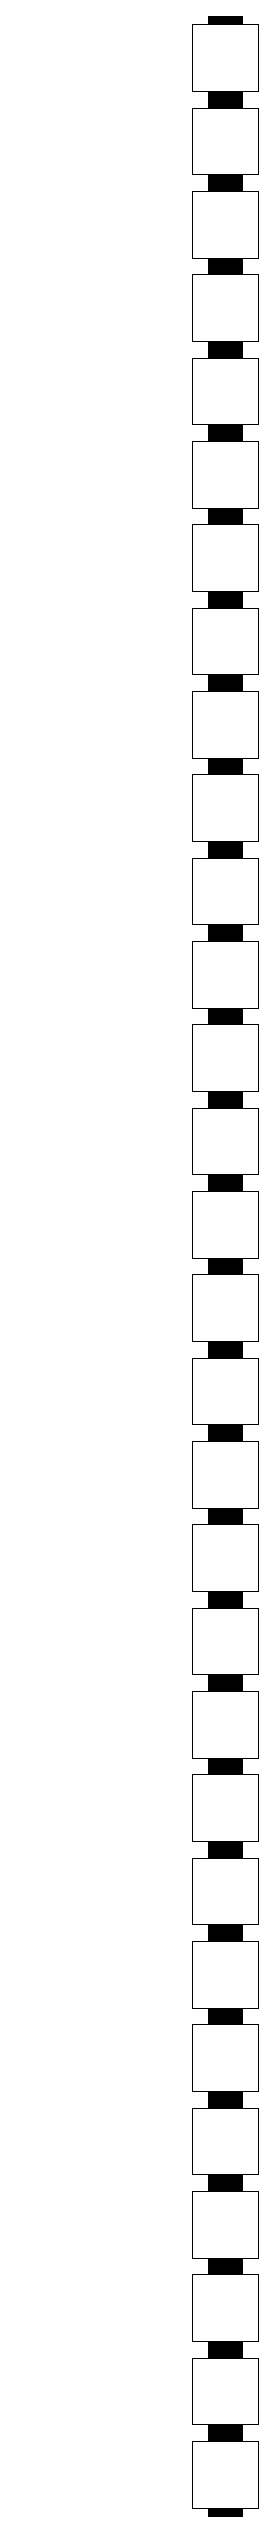
\includegraphics[width=0.2\textwidth]{warping/pre_warp_case2_digit2_msr}
                \caption{\label{fig:warping/pre_warp_case2_digit2_msr} Digit 2 -- Case 2}
            \end{subfigure}%
            ~
            \caption{\label{fig:pre_warp_gadgets} {\prewarp} gadgets }
        \end{figure}


        \item A {\firstwarp} connects to a {\warpbridge} gadget in all cases except when it's assembling
              in the MSR and it is digit 1 in case 1 or 2, in which the {\firstwarp} gadget attaches directly
              to a {\postwarp}.

        \begin{itemize}
            \item if MSR has 1 digit and $u$ ends with 11: Create
            $\begin{aligned}[t]
                \firstwarp(& \left\langle {\tt FirstWarp}, i, u, \inc \right\rangle, \\
                           & \left\langle {\tt FirstWarp}, i, u, \inc \right\rangle, \\
                           & \left\langle {\tt PostWarp},  i, u, \inc \right\rangle \;)
            \end{aligned}$
            \vspace{.5cm}


            \item if MSR has 2 digits and $u$ ends with 01: Create
            $\begin{aligned}[t]
                \firstwarp(& \left\langle {\tt FirstWarp}, i, u, \inc \right\rangle, \\
                & \left\langle {\tt FirstWarp},            i, u, \inc \right\rangle, \\
                & \left\langle {\tt PostWarp},             i, u, \inc \right\rangle \;)
            \end{aligned}$
            \vspace{.5cm}


            \item if MSR has 2 digits and $u$ ends with 11: Create
            $\begin{aligned}[t]
                \firstwarp(& \left\langle {\tt FirstWarp}, i, u, \inc \right\rangle, \\
                & \left\langle {\tt FirstWarp},            i, u, \inc \right\rangle, \\
                & \left\langle {\tt WarpBridge},           i, u, \inc \right\rangle \;)
            \end{aligned}$
            \vspace{.5cm}

            \item if MSR has 3 digits or $d$ starts with 00: Create
            $\begin{aligned}[t]
                \firstwarp(& \left\langle {\tt FirstWarp},  i, u, \inc \right\rangle, \\
                           & \left\langle {\tt FirstWarp},  i, u, \inc \right\rangle, \\
                           & \left\langle {\tt WarpBridge}, i, u, \inc \right\rangle \;)
            \end{aligned}$

        \end{itemize}
        \vspace{.5cm}

        \item A {\warpbridge} gadget binds the last tile of the {\firstwarp} gadgets to the
             first tile of the {\secondwarp} gadgets. For digit 1 in cases 1 and 2, the
             {\warpbridge} is omitted from the {\warpunit}.

        \begin{itemize}
            \item Create
            $\begin{aligned}[t]
                \warpbridge(& \left\langle {\tt WarpBridge}, i, u, \inc \right\rangle, \\
                            & \left\langle {\tt SecondWarp}, i, u, \inc \right\rangle \;)
            \end{aligned}$
            \vspace{.5cm}
        \end{itemize}

        \begin{figure}[H]
            \centering
            \begin{subfigure}[t]{0.2\textwidth}
                \centering
                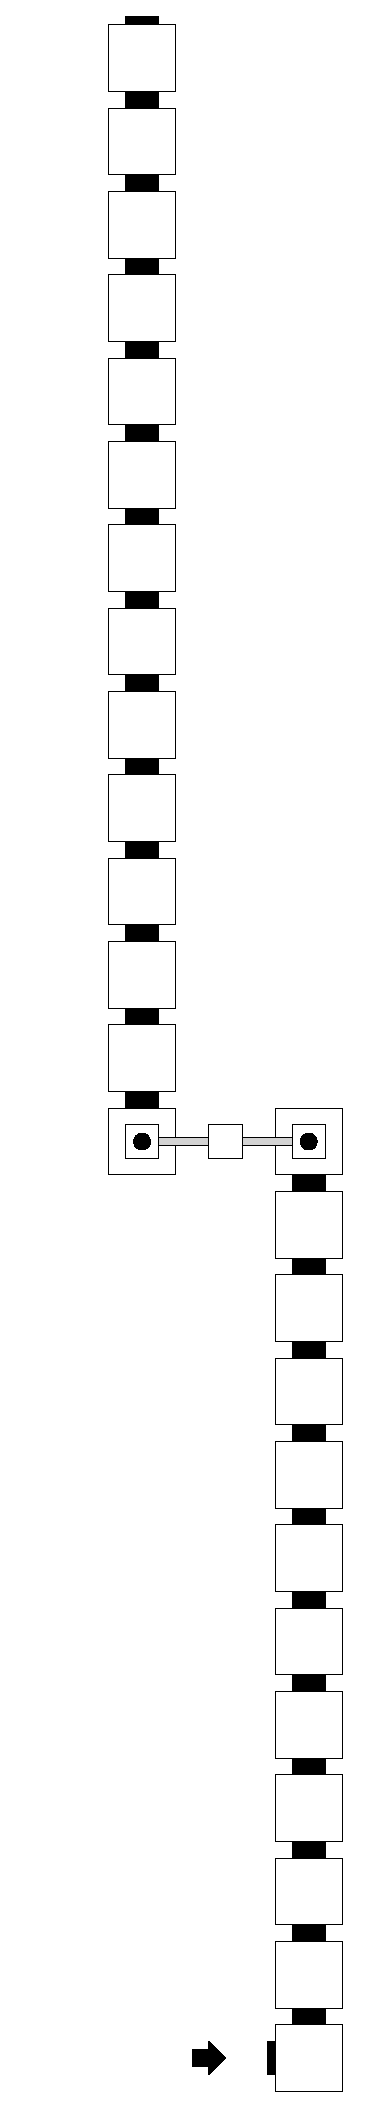
\includegraphics[width=0.2\textwidth]{warping/warp_bridge_general}
                \caption{\label{fig:warping/warp_bridge_general} General}
            \end{subfigure}%
            ~
            \begin{subfigure}[t]{0.2\textwidth}
                \centering
                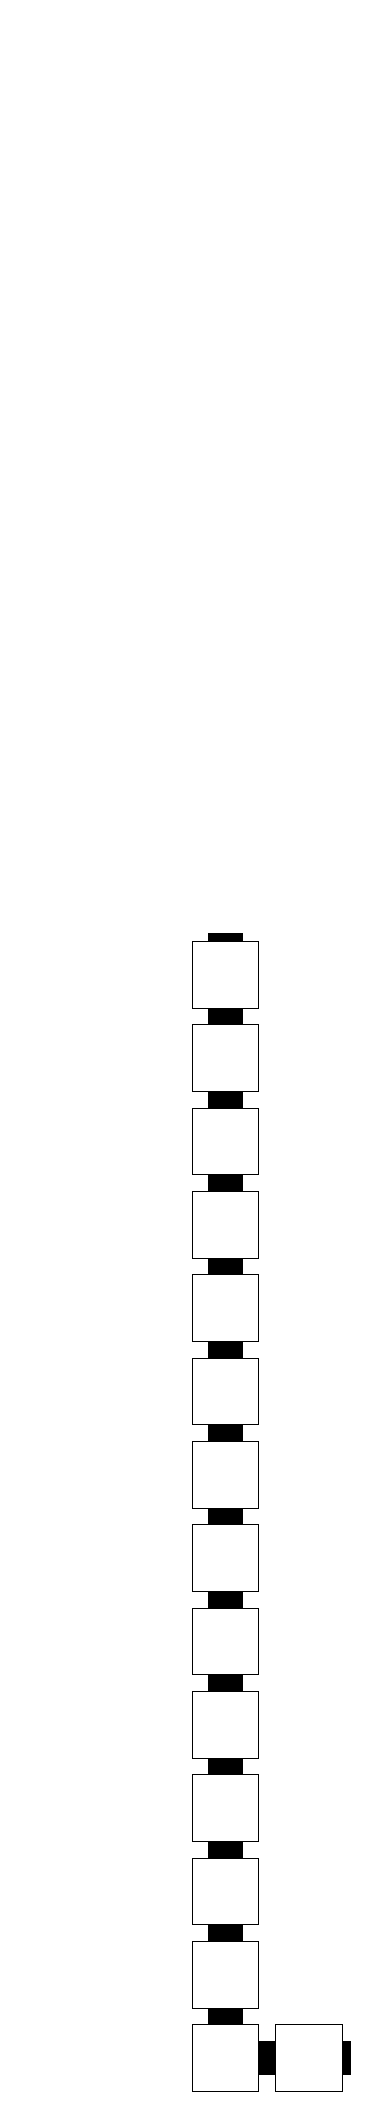
\includegraphics[width=0.2\textwidth]{warping/warp_bridge_case2_digit2_msr}
                \caption{\label{fig:warping/warp_bridge_case2_digit2_msr} Digit 2 -- Case 2}
            \end{subfigure}%
            ~
        \end{figure}




        \item
        Create
        $\begin{aligned}[t]
            \secondwarp(& \left\langle {\tt SecondWarp}, i, u, \inc \right\rangle, \\
                        & \left\langle {\tt SecondWarp}, i, u, \inc \right\rangle, \\
                        & \left\langle {\tt PostWarp},   i, u, \inc \right\rangle \;)
        \end{aligned}$


        \item
        Create
        $\begin{aligned}[t]
            \postwarp(& \left \langle {\tt PostWarp},    i, u, \inc \right\rangle, \\
                      & \left \langle {\tt DigitWriter}, i, u, \inc \right\rangle \;)
        \end{aligned}$

        \begin{figure}[H]
            \begin{subfigure}[t]{0.2\textwidth}
                \centering
                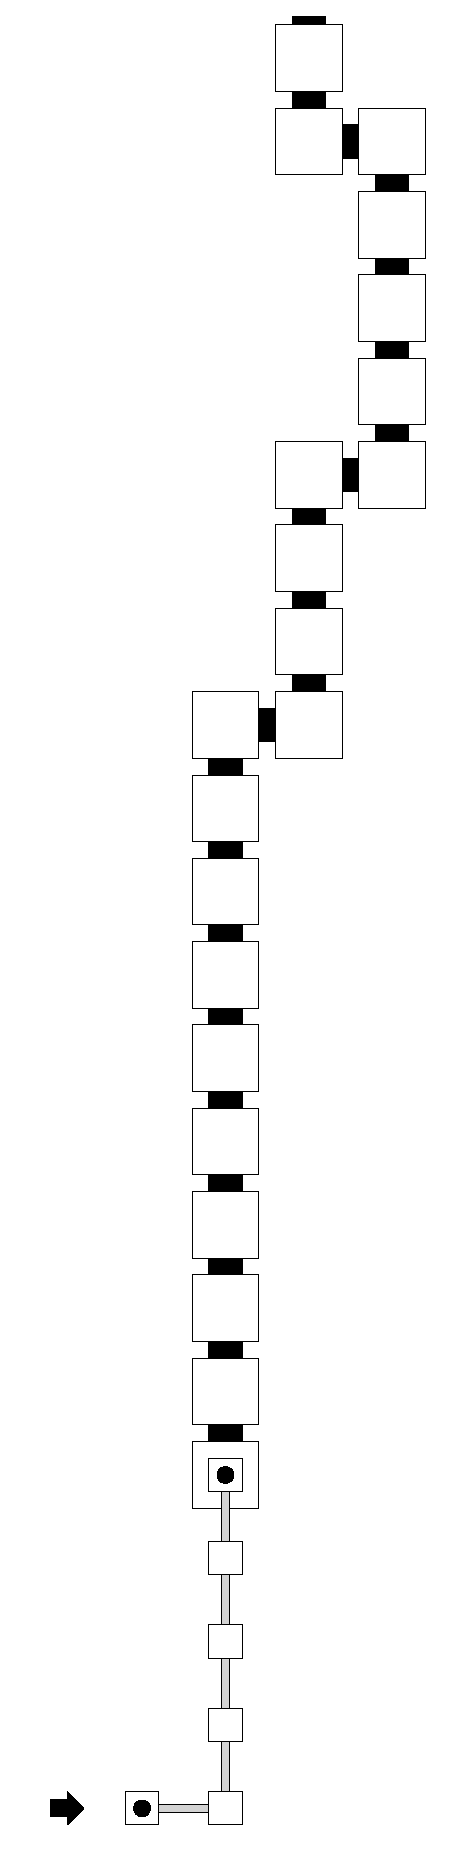
\includegraphics[width=0.2\textwidth]{warping/post_warp_general_digit1}
                \caption{\label{fig:warping/post_warp_general_digit1} General Digit 1}
            \end{subfigure}%
            ~
            \begin{subfigure}[t]{0.2\textwidth}
                \centering
                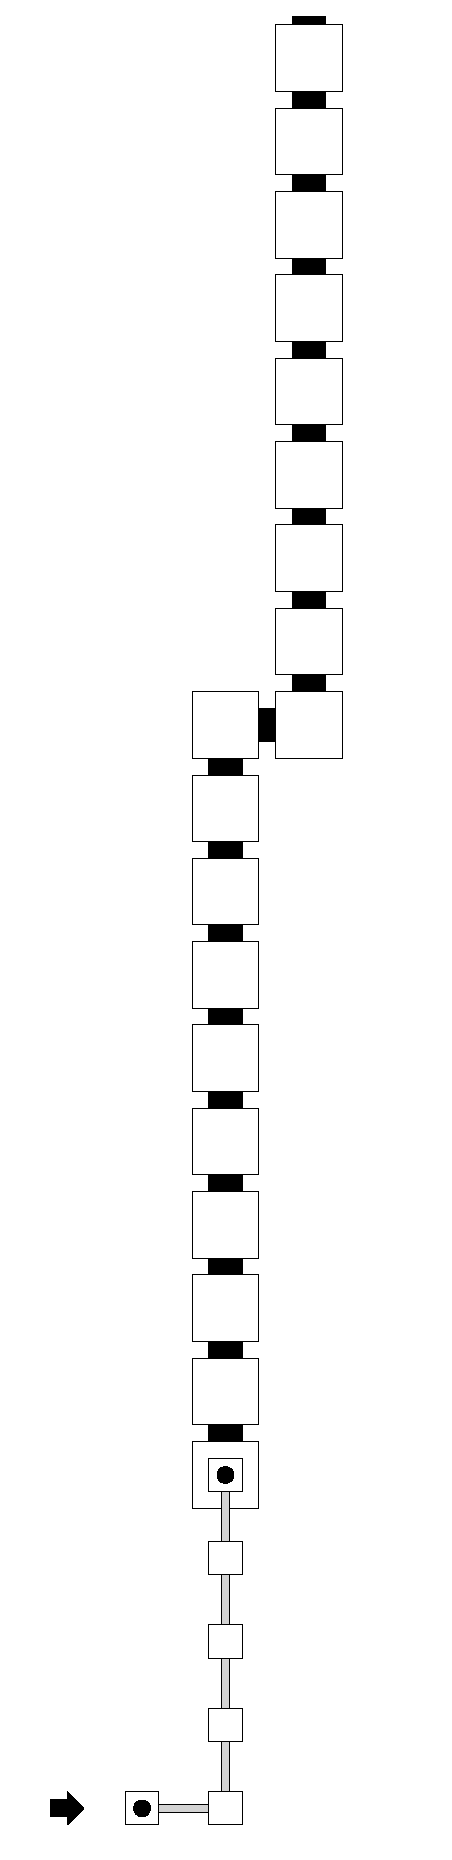
\includegraphics[width=0.2\textwidth]{warping/post_warp_general_digit2and3}
                \caption{\label{fig:warping/post_warp_general_digit2and3} General Digits 2 and 3 }
            \end{subfigure}%
            ~
            \begin{subfigure}[t]{0.2\textwidth}
                \centering
                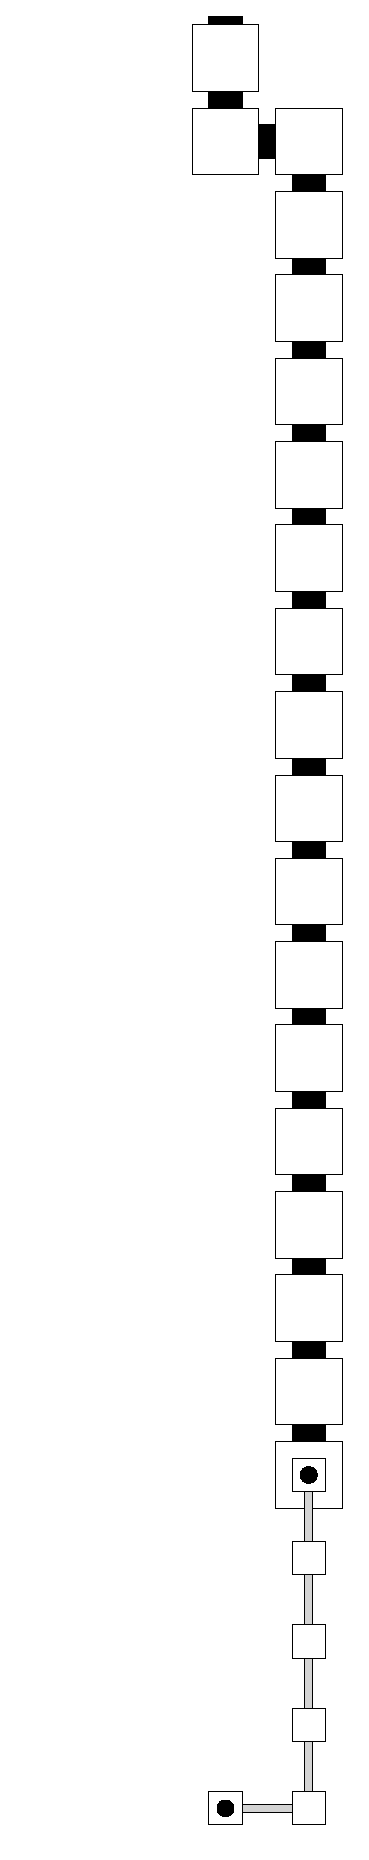
\includegraphics[width=0.2\textwidth]{warping/post_warp_case1_digit1_msr}
                \caption{\label{fig:warping/post_warp_case1_digit1_msr} Digit 1 -- Case 1}
            \end{subfigure}%
            ~
            \begin{subfigure}[t]{0.2\textwidth}
                \centering
                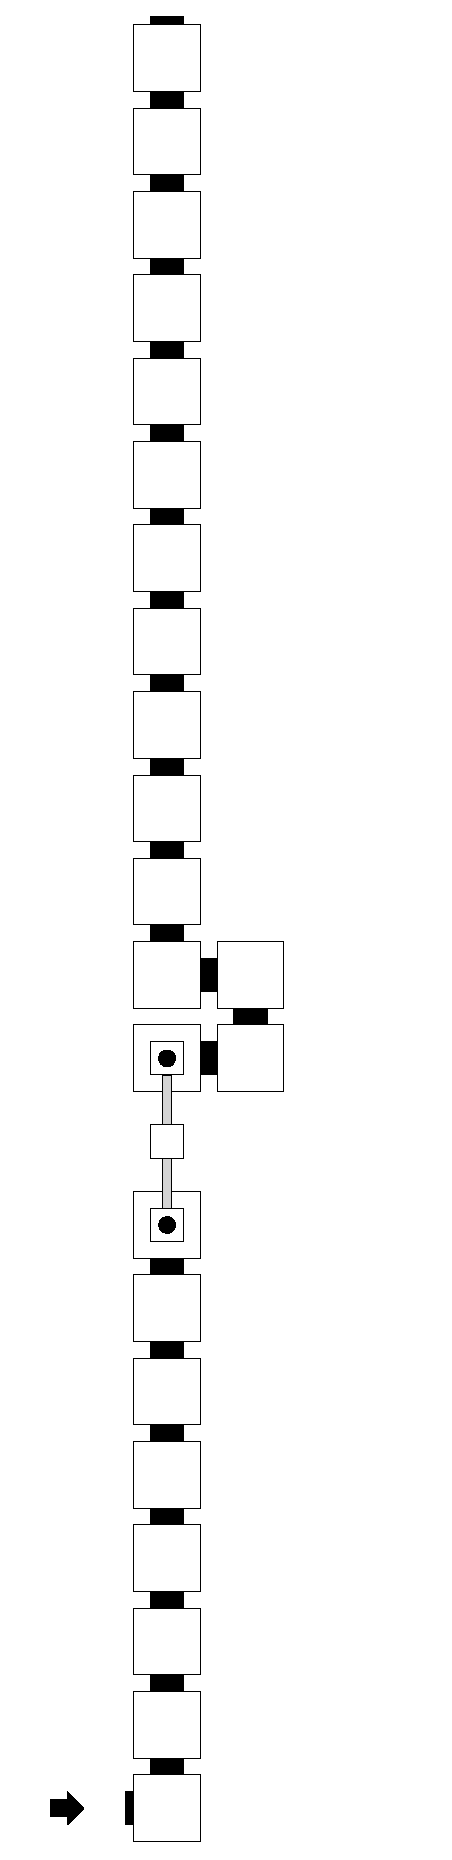
\includegraphics[width=0.2\textwidth]{warping/post_warp_case2_digit1_msr}
                \caption{\label{fig:warping/post_warp_case2_digit1_msr} Digit 1 -- Case 2}
            \end{subfigure}%
            ~

            \begin{subfigure}[t]{0.2\textwidth}
                \centering
                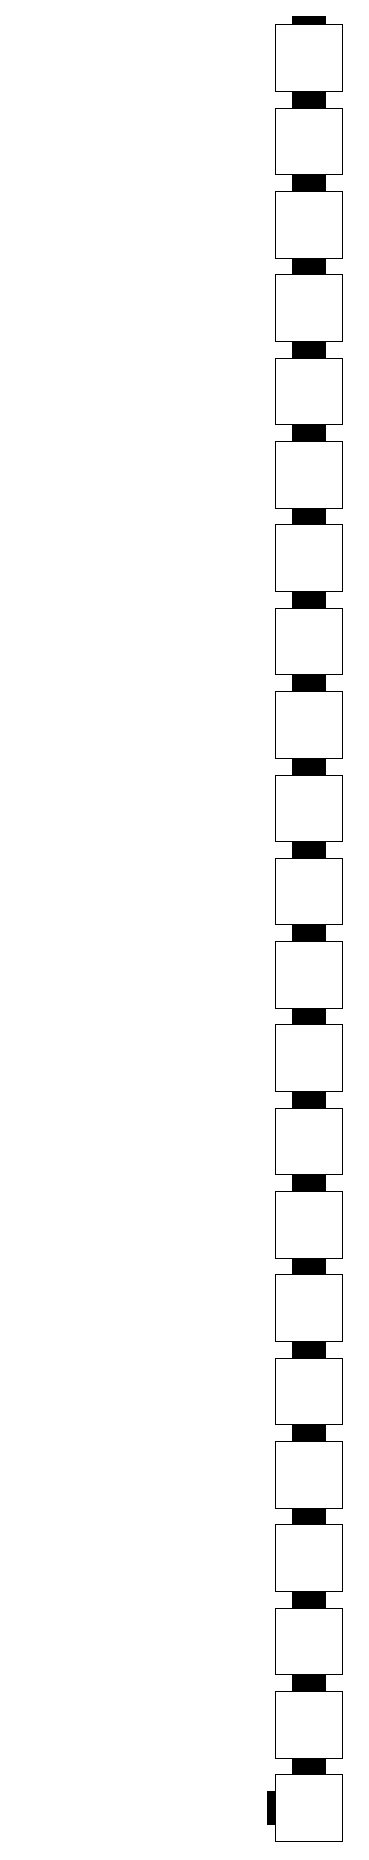
\includegraphics[width=0.2\textwidth]{warping/post_warp_case2_digit2_msr}
                \caption{\label{fig:warping/post_warp_case2_digit2_msr} Digit 2 -- Case 2}
            \end{subfigure}%
            ~
            \caption{\label{fig:post_warp_gadgets} {\postwarp} gadgets }
        \end{figure}

    \end{itemize}



    % For each digit length L
    \subsubsection{ Digit writers }
        % For each index in 1, 2, 3, and carry in 0,1

        \begin{itemize}

            \item For each $i = 1,2,3$,
                           $j = l-1,\ldots,1$,
                           $u \in \{0, 1\}^j$, and
                           $\inc \in \{{\tt increment}, {\tt copy} \}$:
                \begin{itemize}
                \item Create
                    $\begin{aligned}[t]
                        \dwriter(& \left\langle {\tt DigitWriter}, i, u0, \inc \right\rangle, \\
                                & \left\langle {\tt DigitWriter},  i, u,  \inc \right\rangle \;)
                    \end{aligned}$

                \item Create
                $\begin{aligned}[t]
                    \dwriter(& \left\langle {\tt DigitWriter},    i,  u1, \inc \right\rangle, \\
                                & \left\langle {\tt DigitWriter}, i,  u,  \inc \right\rangle \;)
                \end{aligned}$

                \end{itemize}

            \item For each $i = 1,2,3$ and each $\inc \in \{{\tt increment}, {\tt copy} \}$:
            \begin{itemize}
                \item Create
                    $\begin{aligned}[t]
                        \dwriter(& \left\langle {\tt DigitWriter}, i, 0, \inc \right\rangle, \\
                                 & \left\langle {\tt DigitTop}, i, \inc \right\rangle \;)
                    \end{aligned}$

                \item Create
                $\begin{aligned}[t]
                    \dwriter(& \left\langle {\tt DigitWriter}, i, 1, \inc\right\rangle, \\
                             & \left\langle {\tt DigitTop},    i,    \inc\right\rangle \;)
                \end{aligned}$
                \end{itemize}


        \end{itemize}

        \vspace{.5cm}

        \begin{figure}[H]
            \centering
            \begin{subfigure}[t]{0.2\textwidth}
                \centering
                
\includegraphics[width=0.2\textwidth]{write/write_0}
                \caption{\label{fig:write/write_1} Counter\_Write\_0}
            \end{subfigure}%
            ~
            \begin{subfigure}[t]{0.2\textwidth}
                \centering
                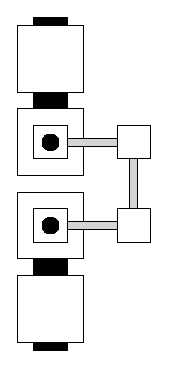
\includegraphics[width=0.2\textwidth]{write/write_1}
                \caption{\label{fig:write/write_1} Counter\_Write\_1}
            \end{subfigure}%
        \end{figure}

    \subsubsection{Digit tops}
        The {\dtop} gadgets have specific geometry, such that they allow {\firstwarp} and
        {\secondwarp} units to ``wake up" and end their warp journey. A {\dtop} is placed on
        the north end of a digit. These hold a increment/copy signal and the regional index
        of the next digit to read.
        \vspace{1cm}

        For each {\inc} $\in \{ {\tt increment, copy } \}$
        \begin{itemize}
            \item General digit tops common to all assemblies

            \begin{figure}[H]
                \centering
                \begin{subfigure}[t]{0.2\textwidth}
                    \centering
                    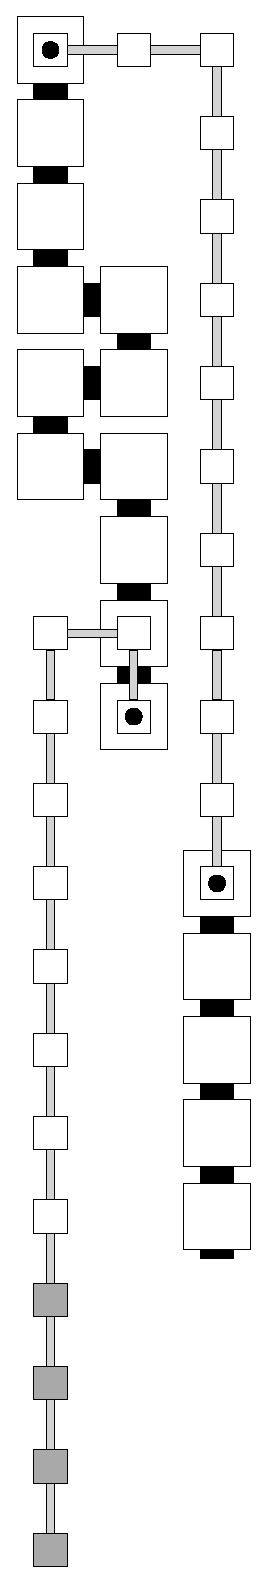
\includegraphics[width=0.2\textwidth]{digit_tops/digit_top_general}
                    \caption{\label{fig:digit_tops/digit_top_general} General }
                \end{subfigure}%
                ~
            \end{figure}

            \begin{itemize}
                \item Create
                $\begin{aligned}[t]
                    \dtop(& \left \langle {\tt DigitTopDigit1}, \inc \right\rangle, & \\
                          & \left \langle {\tt ReturnD1ReadD2}, \inc \right\rangle \;)
                \end{aligned}$
                \vspace{.5cm}

                \item Create
                $\begin{aligned}[t]
                    \dtop(& \left \langle {\tt DigitTopDigit2}, \inc \right\rangle, & \\
                          & \left \langle {\tt ReturnD2ReadD3}, \inc \right\rangle \;)
                \end{aligned}$
                \vspace{.5cm}

                \item Create
                $\begin{aligned}[t]
                    \dtop(& \left \langle {\tt DigitTopDigit3}, \inc \right\rangle,  \\
                          & \left \langle {\tt ReturnD3ReadD1}, \inc \right\rangle \;)
                \end{aligned}$

            \end{itemize}


            \item MSR-specific digit tops. The first tile placed in all digit top gadgets is the rightmost, bottommost tile.

            \begin{figure}[H]
                \centering
                \begin{subfigure}[t]{0.2\textwidth}
                    \centering
                    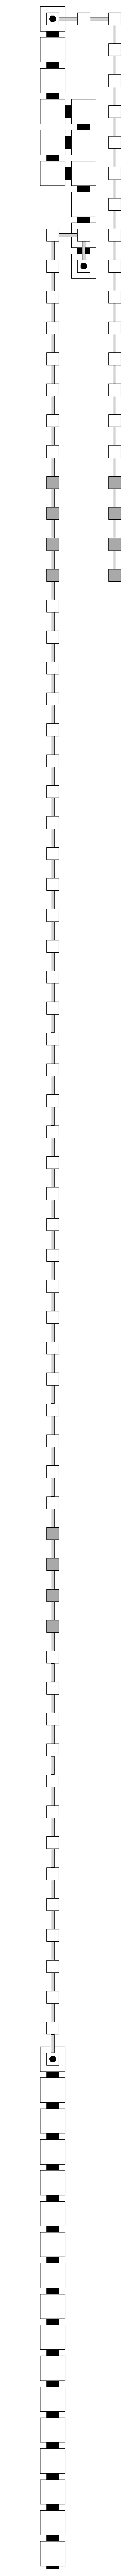
\includegraphics[width=0.2\textwidth]{digit_tops/digit_top_case1_digit1_msr}
                    \caption{\label{fig:digit_tops/digit_top_case1_digit1_msr} Digit 1 -- Case 1}
                \end{subfigure}%
                ~
                \begin{subfigure}[t]{0.2\textwidth}
                    \centering
                    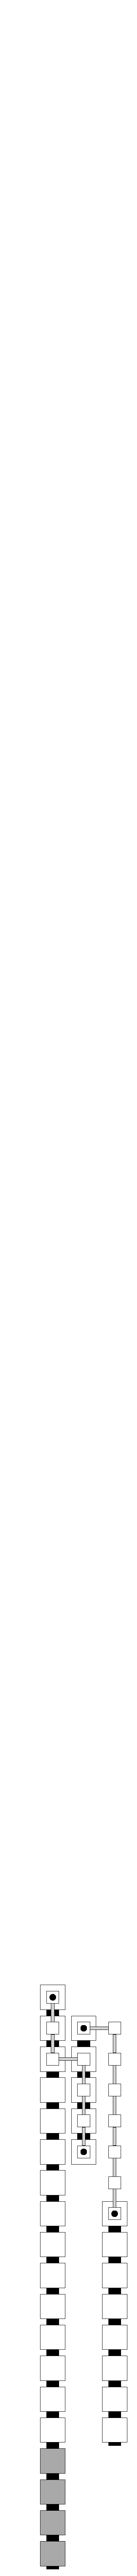
\includegraphics[width=0.2\textwidth]{digit_tops/digit_top_case2_digit1_msr}
                    \caption{\label{fig:digit_tops/digit_top_case2_digit1_msr} Digit 1 -- Case 2}
                \end{subfigure}%
                ~
                \begin{subfigure}[t]{0.2\textwidth}
                    \centering
                    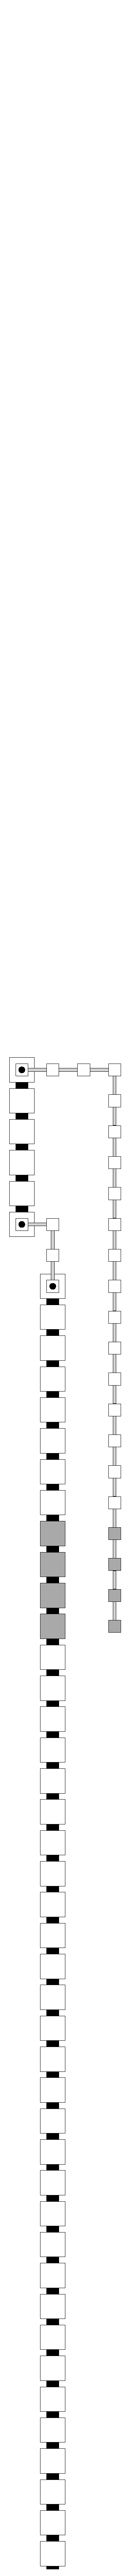
\includegraphics[width=0.2\textwidth]{digit_tops/digit_top_case2_digit2_msr}
                    \caption{\label{fig:digit_tops/digit_top_case2_digit2_msr} Digit 2 -- Case 2}
                \end{subfigure}%
                ~
                \begin{subfigure}[t]{0.2\textwidth}
                    \centering
                    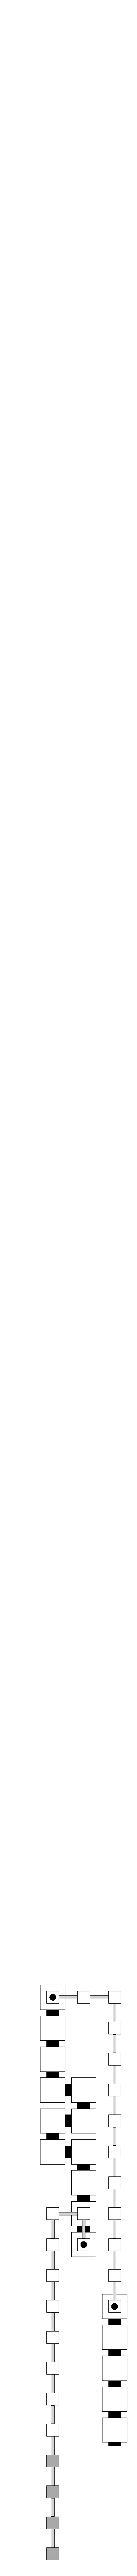
\includegraphics[width=0.2\textwidth]{digit_tops/digit_top_case3_msr}
                    \caption{\label{fig:digit_tops/digit_top_case3_msr} All digits -- Case 3}
                \end{subfigure}%
            \end{figure}


            \begin{enumerate}[label=\alph*)]
                % For digit 1, case 1
                \item if $i$ is 1 and MSR contains 1 digit and $l$ starts with 11:

                Create
                $\begin{aligned}[t]
                    \dtopdonecaseone(& \left \langle {\tt DigitTopDigit1-Case1}, \inc \right\rangle, & \\
                                     & \left \langle {\tt ReturnD1ReadNextRow},  \inc \right\rangle \;)
                \end{aligned}$
                \vspace{.5cm}


                % For digit 1, case 2
                \item if $i$ is 1 and MSR contains 2 digits and $l$ starts with 01:

                Create
                $\begin{aligned}[t]
                    \dtopdonecasetwo(& \left \langle {\tt DigitTopDigit1-Case2}, \inc \right\rangle, & \\
                                     & \left \langle {\tt ReturnD1ReadD2-Case2}, \inc \right\rangle \;)
                \end{aligned}$
                \vspace{.5cm}


                % For digit 2, case 2
                \item if $i$ is 2 and MSR contains 2 digits and $l$ starts with 11:

                Create
                $\begin{aligned}[t]
                    \dtopdtwocasetwo(& \left \langle {\tt DigitTopDigit2-Case2}, \inc \right\rangle, & \\
                                     & \left \langle {\tt ReturnD2ReadNextRow},  \inc \right\rangle \;)
                \end{aligned}$
                \vspace{.5cm}


                % For digit 3, in case 3
                \item if $i$ is 3 and MSR contains 3 digits and $l$ starts with 11:

                Create
                $\begin{aligned}[t]
                    \dtopcasethree(& \left \langle {\tt DigitTop-Case3},      \inc \right\rangle, & \\
                                   & \left \langle {\tt ReturnD3ReadNextRow}, \inc \right\rangle \;)
                \end{aligned}$
                \vspace{.5cm}


            \end{enumerate}

        \end{itemize}
    \vspace{1cm}



    \subsubsection{Return paths between the MSD and LSD in different rows}

        The gadgets of this class hold a increment/copy signal.
        The height of these gadgets is dependent on $l$ and the width is dependent of $k$.
        These gadgets are used to begin reading the first digit in the following row, once
        the MSD has been read in the current row.
        \vspace{1cm}

        \begin{figure}[H]
            \centering
            \begin{subfigure}[t]{0.3\textwidth}
                \centering
                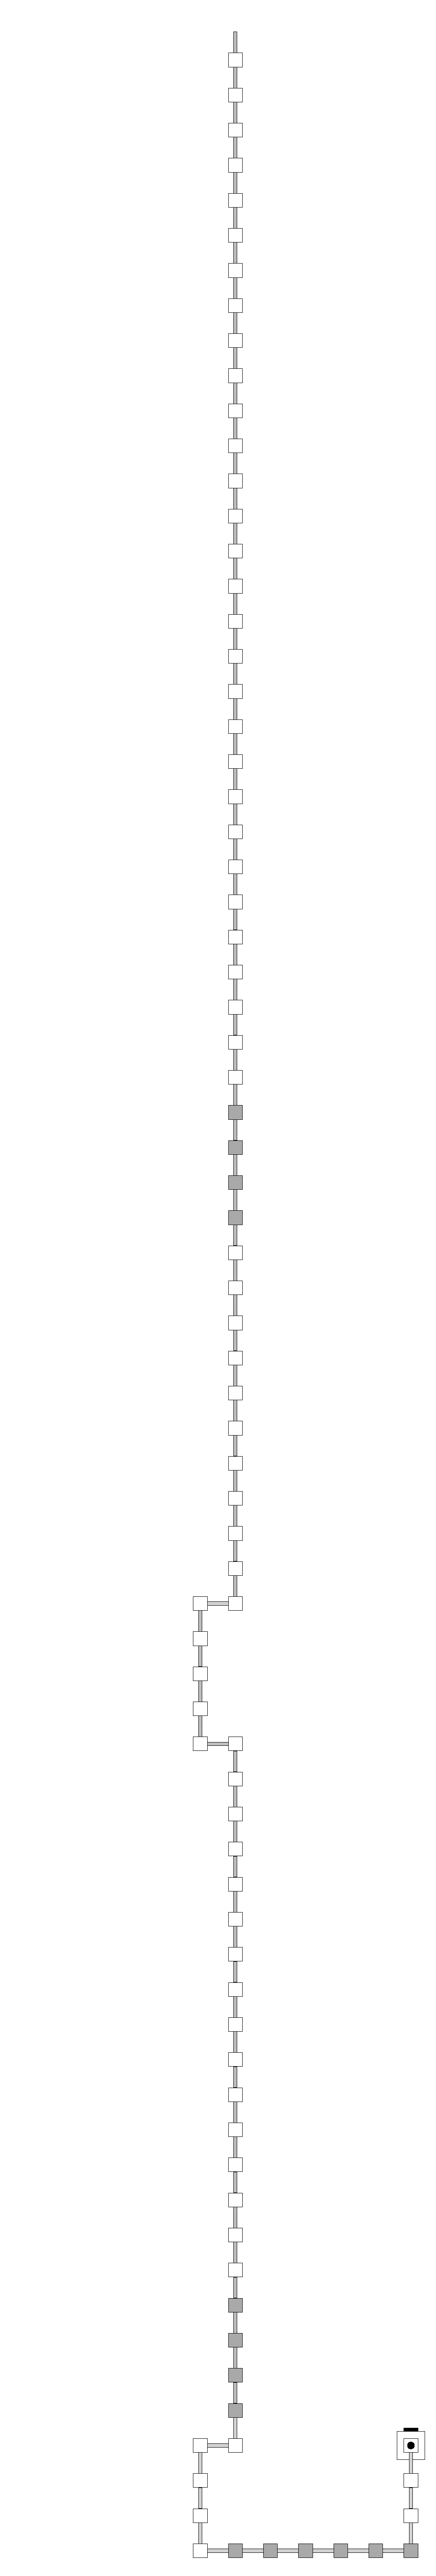
\includegraphics[width=0.3\textwidth]{return_paths/return_digit1_read_next_row}
                \caption{\label{fig:return_paths/return_digit1_read_next_row} Case -- 1}
            \end{subfigure}%
            ~
            \begin{subfigure}[t]{0.3\textwidth}
                \centering
                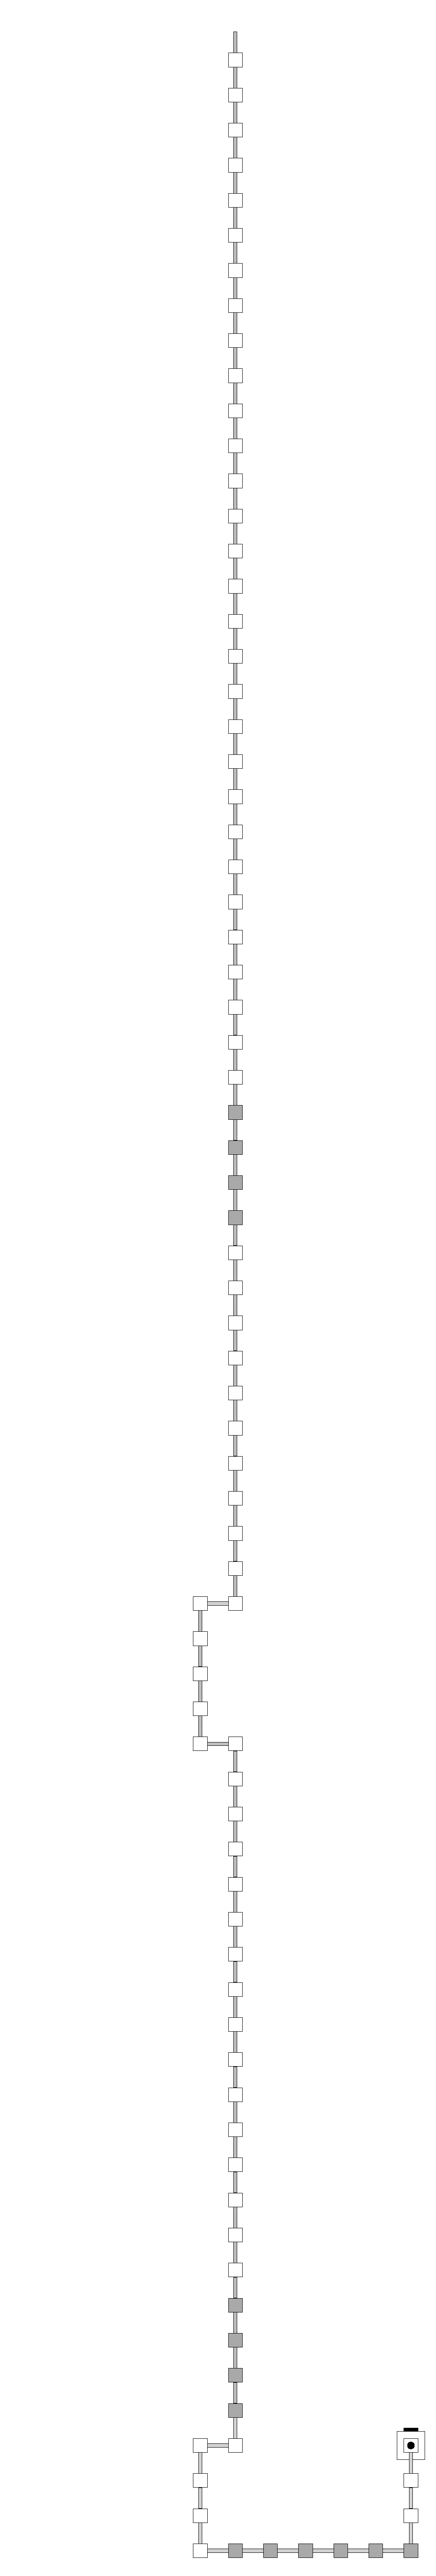
\includegraphics[width=0.3\textwidth]{return_paths/return_digit2_read_next_row}
                \caption{\label{fig:return_paths/return_digit2_read_next_row} Case -- 2}
            \end{subfigure}%
            ~
            \begin{subfigure}[t]{0.3\textwidth}
                \centering
                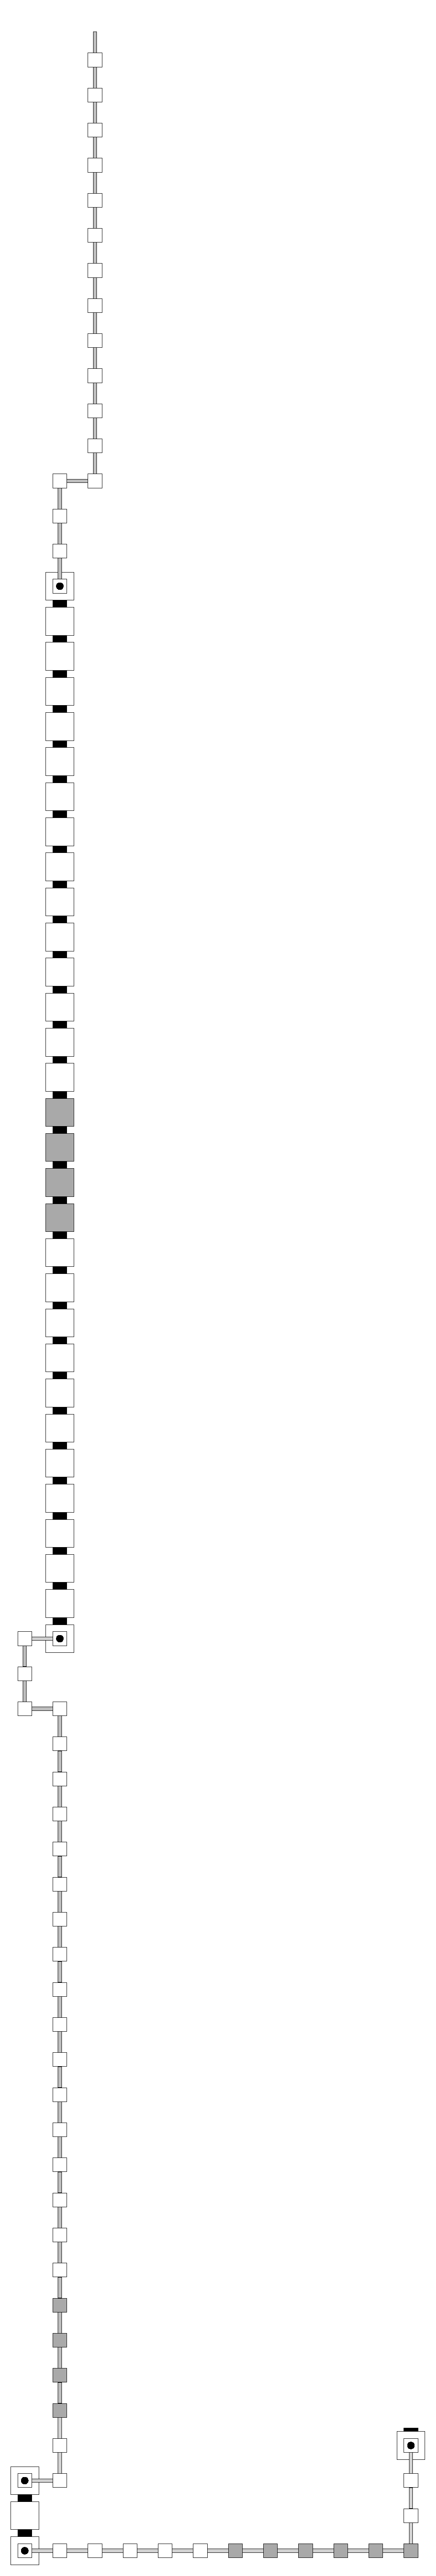
\includegraphics[width=0.3\textwidth]{return_paths/return_digit3_read_next_row}
                \caption{\label{fig:return_paths/return_digit3_read_next_row} Case -- 3}
            \end{subfigure}%
            \caption{\label{fig:return_path_next_row}
            All of these gadgets assemble north to south. The vertical gray lines tiles have a height
            that depends on $l$ and the horizontal gray lines depend on $k$. (cases 1 and 2 are geometrically equivalent)}
        \end{figure}


        \noindent For each {\inc} $\in \{ {\tt increment, copy } \}$

        \begin{itemize}
            \item Create
            $\begin{aligned}[t]
                \returnfromdonereadnextrow(& \left \langle {\tt ReturnD1ReadNextRow},     \inc \right\rangle, & \\
                                           & \left \langle {\tt DigitReader}, 1, \lambda, \inc \right\rangle \;)
            \end{aligned}$

            \item Create
            $\begin{aligned}[t]
                \returnfromdtworeadnextrow(& \left \langle {\tt ReturnD2ReadNextRow},     \inc \right\rangle, & \\
                                           & \left \langle {\tt DigitReader}, 1, \lambda, \inc \right\rangle \;)
            \end{aligned}$

            \item Create
            $\begin{aligned}[t]
                \returnfromdthreereadnextrow(& \left \langle {\tt ReturnD3ReadNextRow},     \inc \right\rangle, & \\
                                             & \left \langle {\tt DigitReader}, 1, \lambda, \inc \right\rangle \;)
            \end{aligned}$
        \end{itemize}
    \vspace{1cm}



    \subsubsection{Return paths between digits in the same row}
        The gadgets of this class hold a increment/copy signal and the regional index
        of the next digit to read. The height of these gadgets is dependent on $l$.
        These gadgets are used so that upon writing a digit, the counter
        is able to move back down to the next digit in the current row, and continue
        reading.
        \vspace{1cm}

        \begin{figure}[H]
            \centering
            \begin{subfigure}[t]{0.2\textwidth}
                \centering
                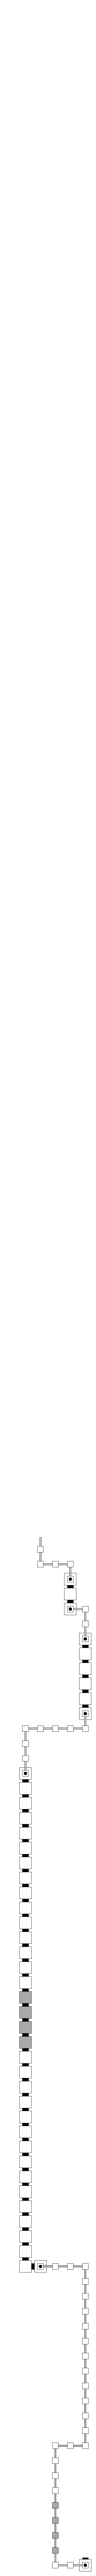
\includegraphics[width=0.2\textwidth]{return_paths/return_digit1_read_digit2_general}
                \caption{\label{fig:return_paths/return_digit1_read_digit2_general} Return digit 1 read digit 2}
            \end{subfigure}%
            ~
            \begin{subfigure}[t]{0.2\textwidth}
                \centering
                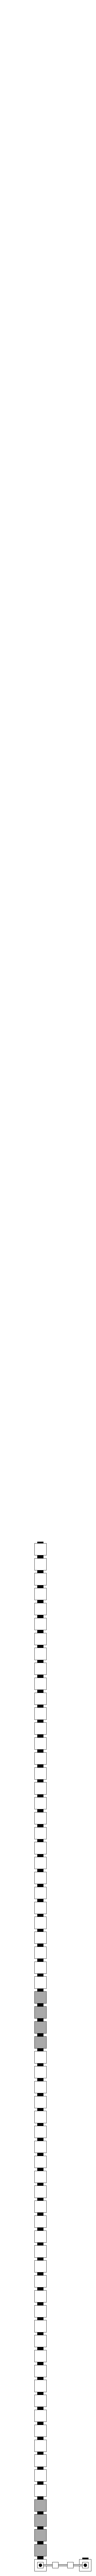
\includegraphics[width=0.2\textwidth]{return_paths/return_digit1_read_digit2_case2_msr}
                \caption{\label{fig:return_paths/return_digit1_read_digit2_case2_msr} Return digit 1 read digit 2 -- Case 2}
            \end{subfigure}%
            ~
            \begin{subfigure}[t]{0.2\textwidth}
                \centering
                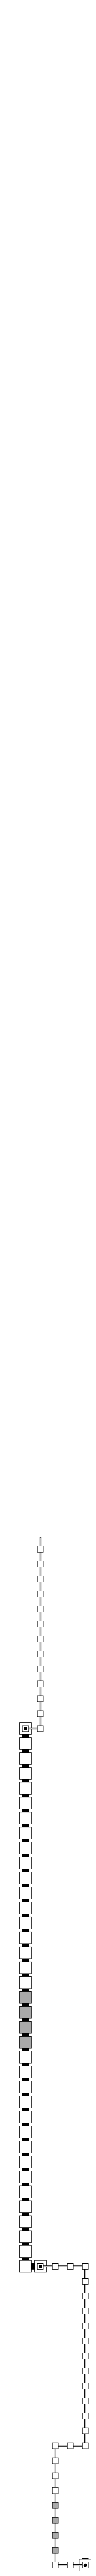
\includegraphics[width=0.2\textwidth]{return_paths/return_digit2_read_digit3_general}
                \caption{\label{fig:return_paths/return_digit2_read_digit3_general} Return digit 2 read digit 3}
            \end{subfigure}%
            ~
            \begin{subfigure}[t]{0.2\textwidth}
                \centering
                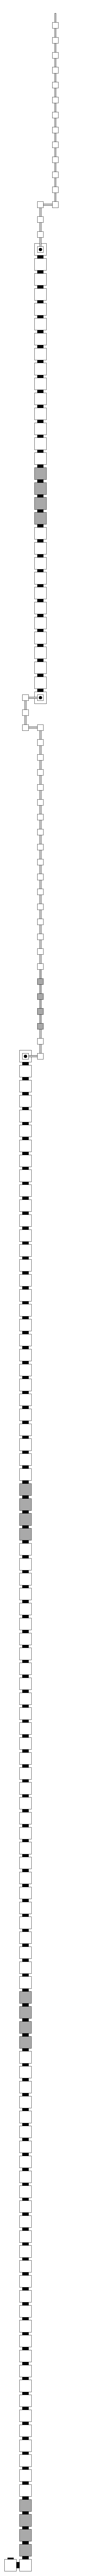
\includegraphics[width=0.2\textwidth]{return_paths/return_digit3_read_digit1_general}
                \caption{\label{fig:return_paths/return_digit1_read_digit2_general} Return digit 3 read digit 1}
            \end{subfigure}%
            \caption{\label{fig:return_path_same_row} All of these gadgets grow from north to south, the height of gray tiles depends on $l$.}
        \end{figure}

        \noindent For each {\inc} $\in \{ {\tt increment, copy } \}$.

        % todo yes/no?: pass L as input since gadget size is O(L), but inputs/outputs don't depend on it

        \begin{itemize}
            \item Create
            $\begin{aligned}[t]
                \returnfromdonereaddtwo(& \left \langle {\tt ReturnD1ReadD2},          \inc \right\rangle, \\
                                        & \left \langle {\tt DigitReader}, 2, \lambda, \inc \right\rangle \;)
            \end{aligned}$

            \item Create
            $\begin{aligned}[t]
                \returnfromdonereaddtwocasetwo(& \left \langle {\tt ReturnD1ReadD2-Case2},    \inc \right\rangle, \\
                                               & \left \langle {\tt DigitReader}, 2, \lambda, \inc \right\rangle \;)
            \end{aligned}$

            \item Create
            $\begin{aligned}[t]
                \returnfromdtworeaddthree(& \left \langle {\tt ReturnD2ReadD3},           \inc \right\rangle, \\
                                          & \left \langle {\tt DigitReader},  3, \lambda, \inc \right\rangle \;)
            \end{aligned}$

            \item Create
            $\begin{aligned}[t]
                 \returnfromdthreereaddone(& \left \langle {\tt ReturnD3ReadD1},           \inc \right\rangle, \\
                                           & \left \langle {\tt DigitReader},  1, \lambda, \inc \right\rangle \;)
            \end{aligned}$

        \end{itemize}


    \subsection{Seed Unit (updated to assemble in a more consistent fashion)}

    \begin{figure}[H]
        \centering
        \begin{subfigure}[t]{0.3\textwidth}
            \centering
            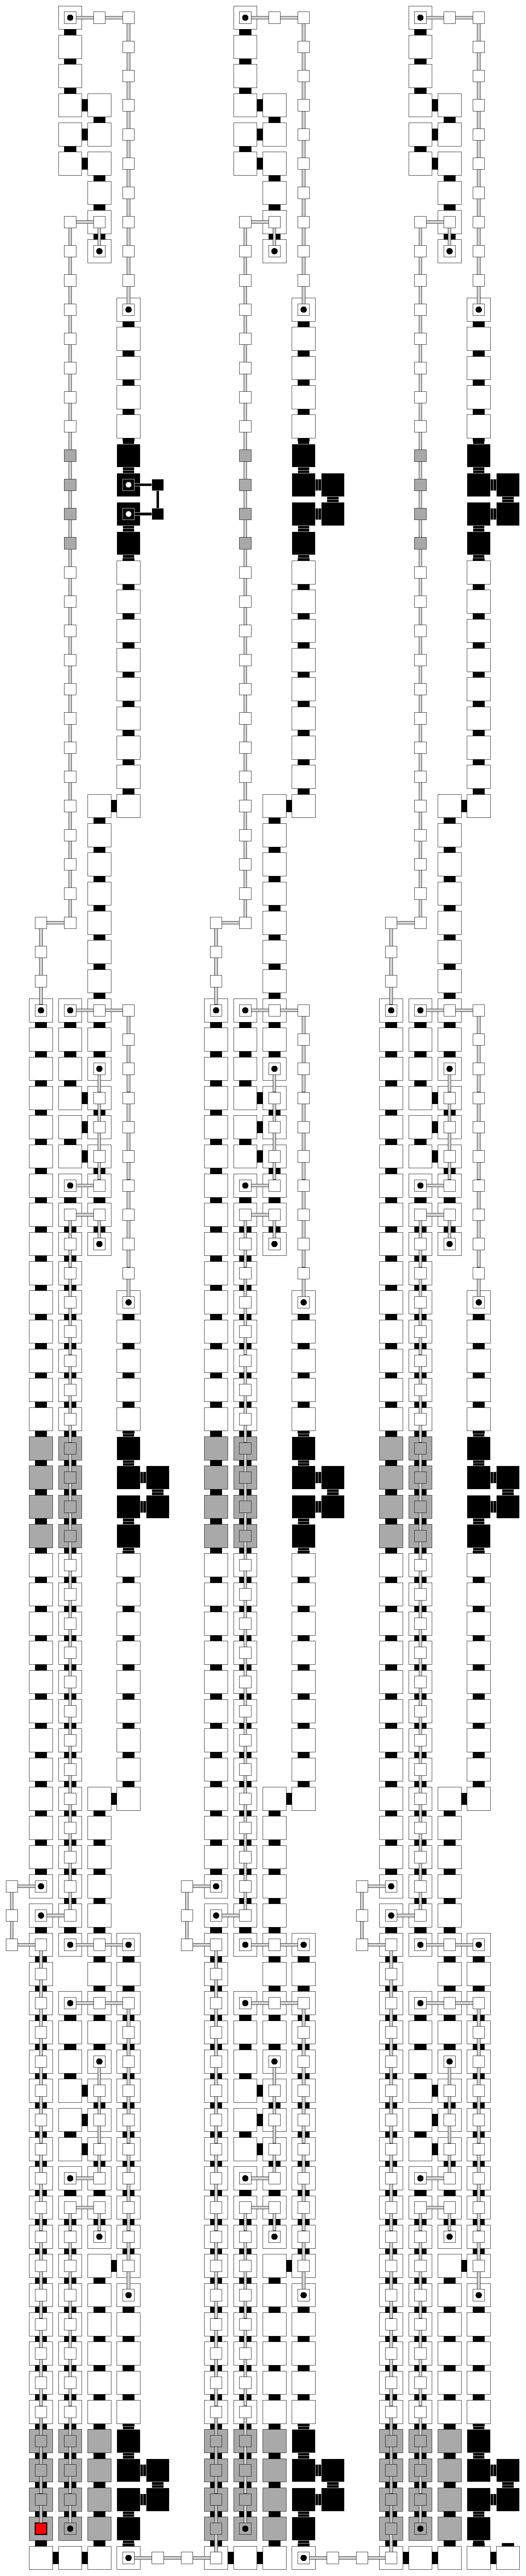
\includegraphics[width=0.3\textwidth]{seed/seed_overview_case3}
            \caption{\label{fig:seed_overview_case3} Initial value case 3}
        \end{subfigure}%
        ~
        \begin{subfigure}[t]{0.3\textwidth}
            \centering
            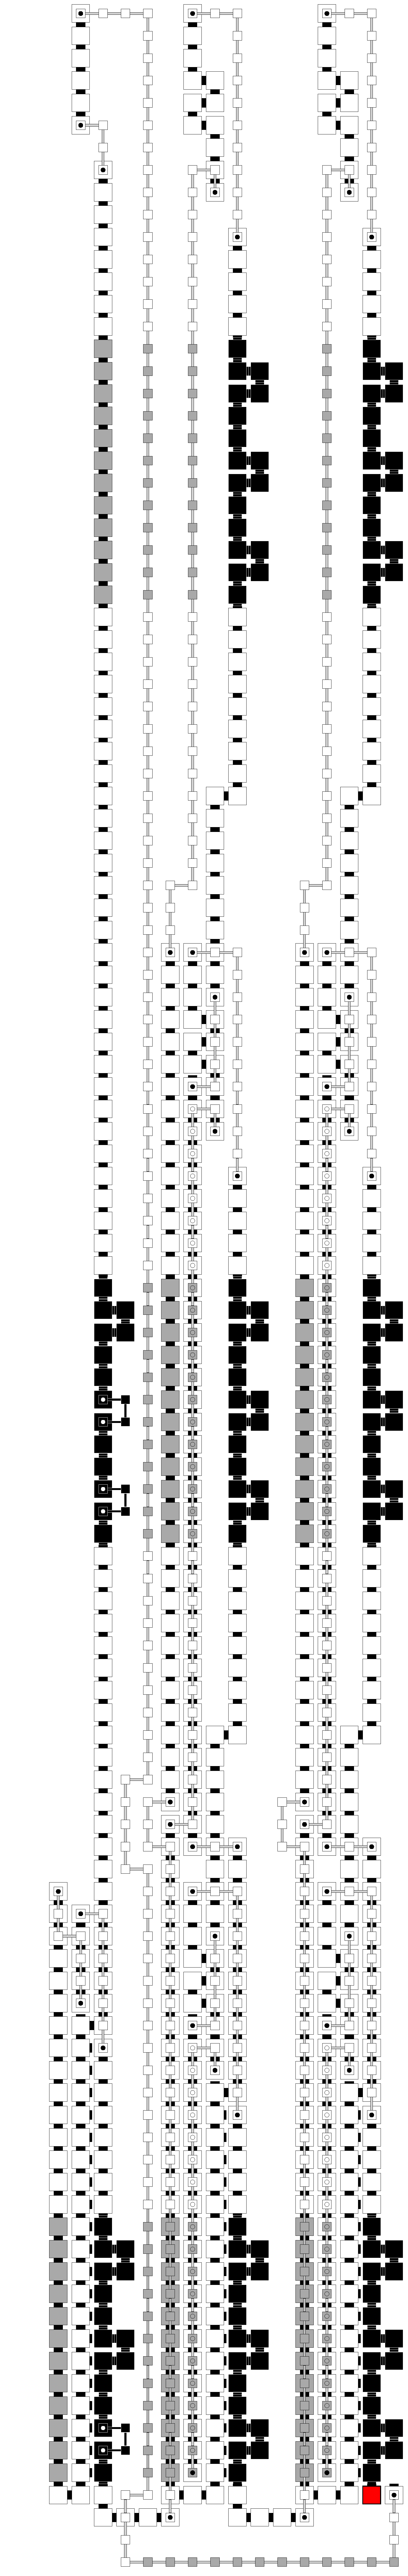
\includegraphics[width=0.3\textwidth]{seed/seed_overview_case2}
            \caption{\label{fig:seed_overview_case2} Initial value case 2}
        \end{subfigure}%
        ~
        \begin{subfigure}[t]{0.3\textwidth}
            \centering
            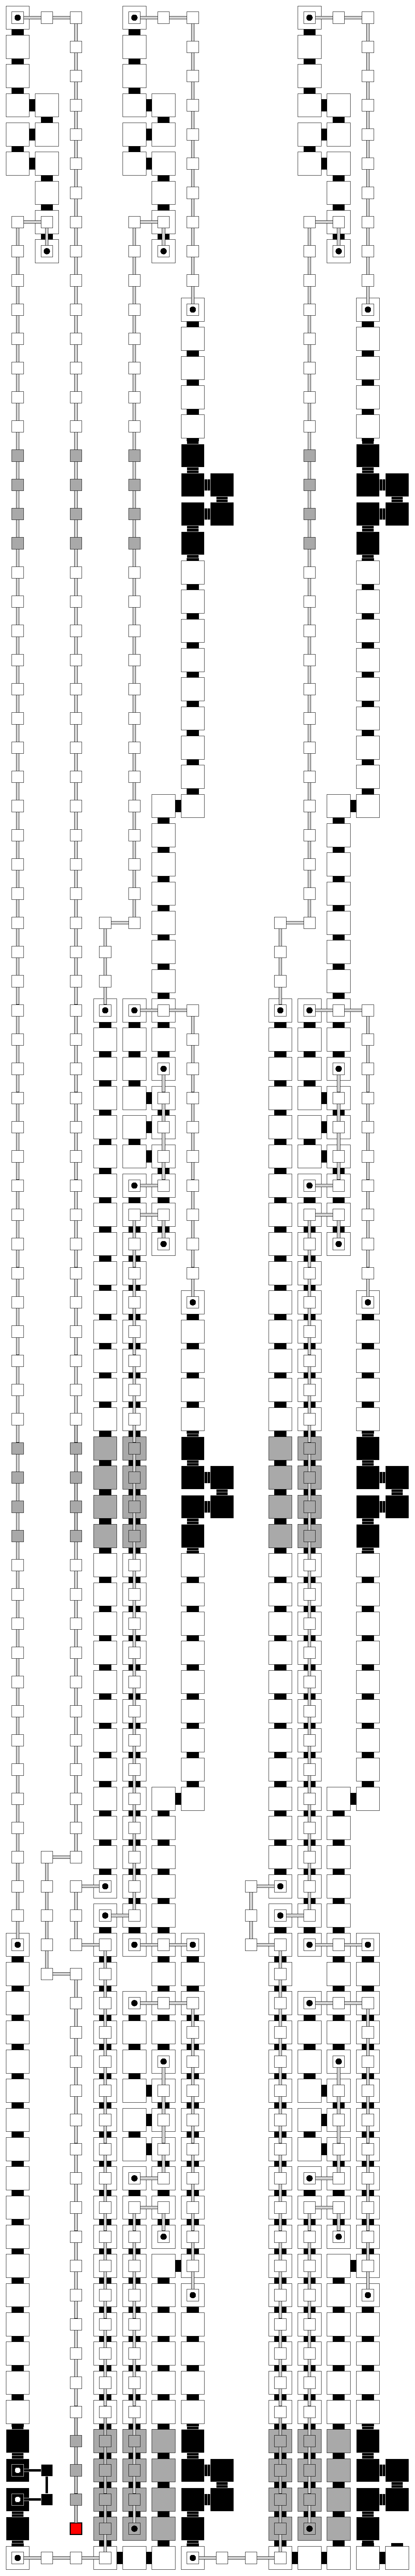
\includegraphics[width=0.3\textwidth]{seed/seed_overview_case1}
            \caption{\label{fig:seed_overview_case1} Initial value case 1}
        \end{subfigure}%
        ~
    \end{figure}

    \subsection{Overviews}

    \begin{figure}[H]
        \centering
        \begin{subfigure}[t]{0.2\textwidth}
            \centering
            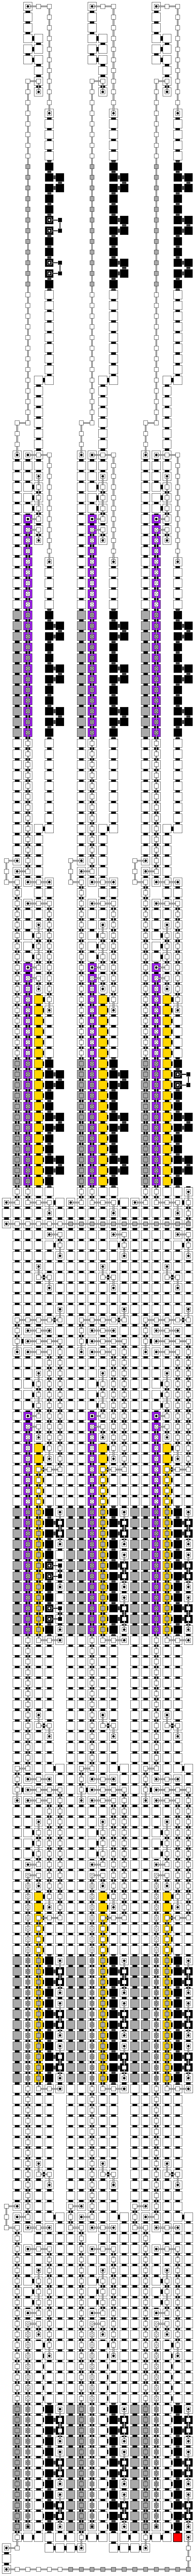
\includegraphics[width=0.2\textwidth]{full_overview_case3_colored}
            \caption{\label{fig:full_overview_case3_colored} Full overview case 3}
        \end{subfigure}%
        ~
        \begin{subfigure}[t]{0.2\textwidth}
            \centering
            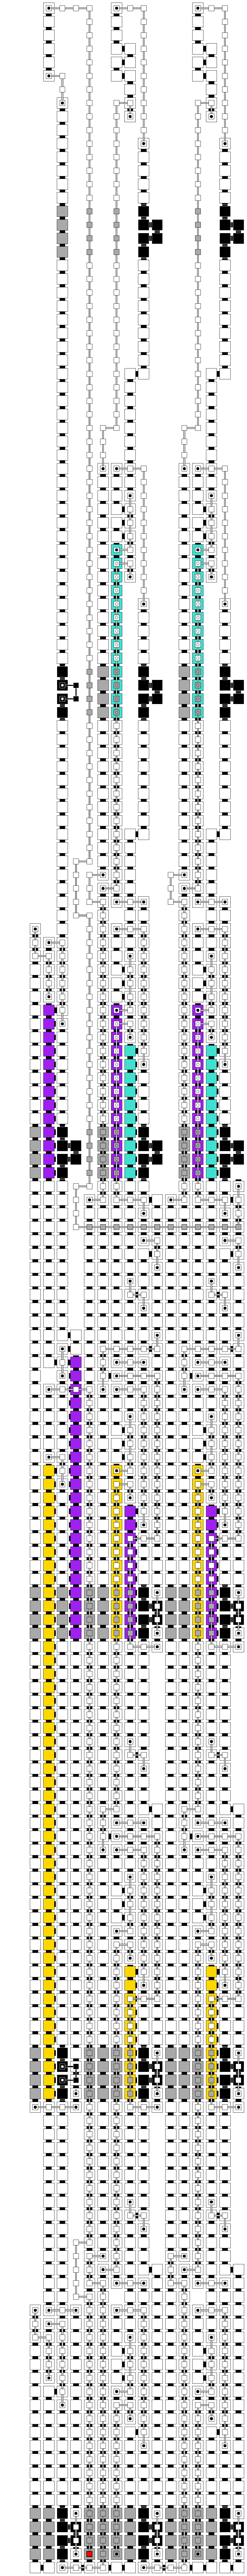
\includegraphics[width=0.2\textwidth]{full_overview_case2_colored}
            \caption{\label{fig:full_overview_case2_colored} Full overview case 2}
        \end{subfigure}%
        ~
        \begin{subfigure}[t]{0.2\textwidth}
            \centering
            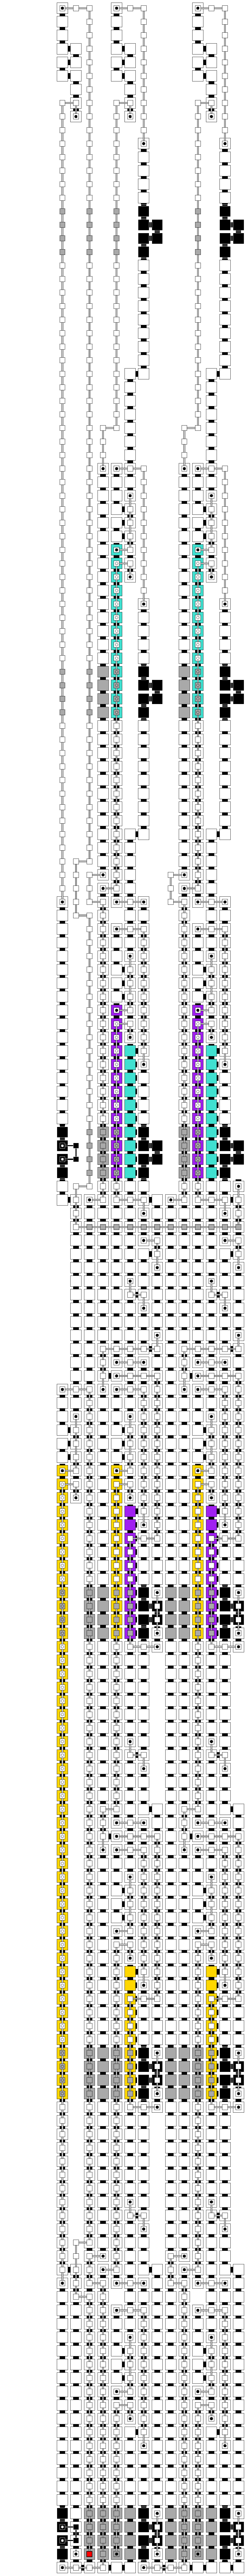
\includegraphics[width=0.2\textwidth]{full_overview_case1_colored}
            \caption{\label{fig:full_overview_case1_colored} Full overview case 1}
        \end{subfigure}%
        ~
    \end{figure}